\section{Experimental Setup}
\label{sec:experimental_setup}

This section describes the experimental design used to evaluate three key components of the proposed calibrated surrogate-assisted optimization framework.

\subsection{Experimental Objectives}
\label{subsec:experimental_objectives}

First, the global surrogate models are evaluated on unseen shear wall layouts. The feasibility surrogate is assessed in terms of both classification performance and conservative screening ability, while the reinforcement surrogate is assessed in terms of prediction accuracy and ranking quality. To verify the role of layout representation, three input settings are compared: design parameters only, design parameters with global layout statistics, and the proposed graph-based layout representation.

Second, the effectiveness of online local calibration is investigated. Since each optimization task is performed for a fixed layout and design condition, FEA-verified samples generated during optimization can provide layout-specific feedback. The calibration experiments therefore examine whether a small number of locally verified samples can improve feasibility probability calibration, reduce reinforcement prediction bias, and improve candidate ranking in the current layout.

Third, the calibrated surrogate models are embedded into optimization procedures. The optimization experiments compare full FEA-based optimization with several surrogate-assisted evaluation strategies. The comparison focuses on the number of true FEA calls, feasible-solution discovery, and final material cost. All compared methods use the same design space and true evaluator.

\begin{table}[t]
\centering
\caption{Sampling space of structural design parameters.}
\label{tab:parameter_space}
\setlength{\tabcolsep}{3pt}
\begin{tabularx}{\columnwidth}{@{}>{\raggedright\arraybackslash}p{0.30\columnwidth}>{\centering\arraybackslash}p{0.17\columnwidth}>{\centering\arraybackslash}p{0.08\columnwidth}>{\raggedright\arraybackslash}X@{}}
\toprule
Parameter & Symbol & Unit & Sampling values \\
\midrule
Number of stories & $N$ & - & 18--33 \\
Story height & $h_{story}$ & m & 2.9 \\
Bottom wall thickness & $t_{w,b}$ & mm & 200, 250, 300, 350, 400 \\
Middle wall thickness & $t_{w,m}$ & mm & 160, 180, 200, 250, 300 \\
Top wall thickness & $t_{w,t}$ & mm & 160, 180, 200, 250 \\
Main beam depth & $h_{m}$ & mm & 400, 500, 550, 600, 650, 700 \\
Main beam width & $b_{m}$ & mm & 200, 250, 300, 350 \\
Secondary beam depth & $h_{s}$ & mm & 300, 400, 450, 500 \\
Secondary beam width & $b_{s}$ & mm & 200, 250, 300 \\
Concrete grade & $f_c$ & - & C30, C35, C40, C45, C50 \\
Seismic intensity & $S_I$ & - & 6.0, 7.0, 7.5, 8.0 \\
Site class & $S_C$ & - & I0, I, II, III, IV \\
Seismic group & $S_G$ & - & 1, 2, 3 \\
\bottomrule
\end{tabularx}
\end{table}

\begin{table*}[t]
\centering
\caption{Dataset split and design-condition groups.}
\label{tab:dataset_split}
\setlength{\tabcolsep}{5pt}
\begin{tabularx}{\textwidth}{@{}>{\raggedright\arraybackslash}p{0.18\textwidth}
>{\centering\arraybackslash}p{0.15\textwidth}
>{\centering\arraybackslash}p{0.16\textwidth}
>{\centering\arraybackslash}X@{}}
\toprule
Subset & No. of layouts & No. of samples & Group ratio (Group7-H1 / Group7-H2 / Group8) \\
\midrule
Training & 100 & 499,977 & 19.0\% / 38.0\% / 43.0\% \\
Validation & 22  & 109,996 & 33.3\% / 47.6\% / 19.0\% \\
Testing & 21 & 104,999 & 31.8\% / 18.2\% / 50.0\% \\
\midrule
Total & 143 & 714,972 & 23.1\% / 36.4\% / 40.6\% \\
\bottomrule
\end{tabularx}
\end{table*}


\begin{figure*}[t]
\centering
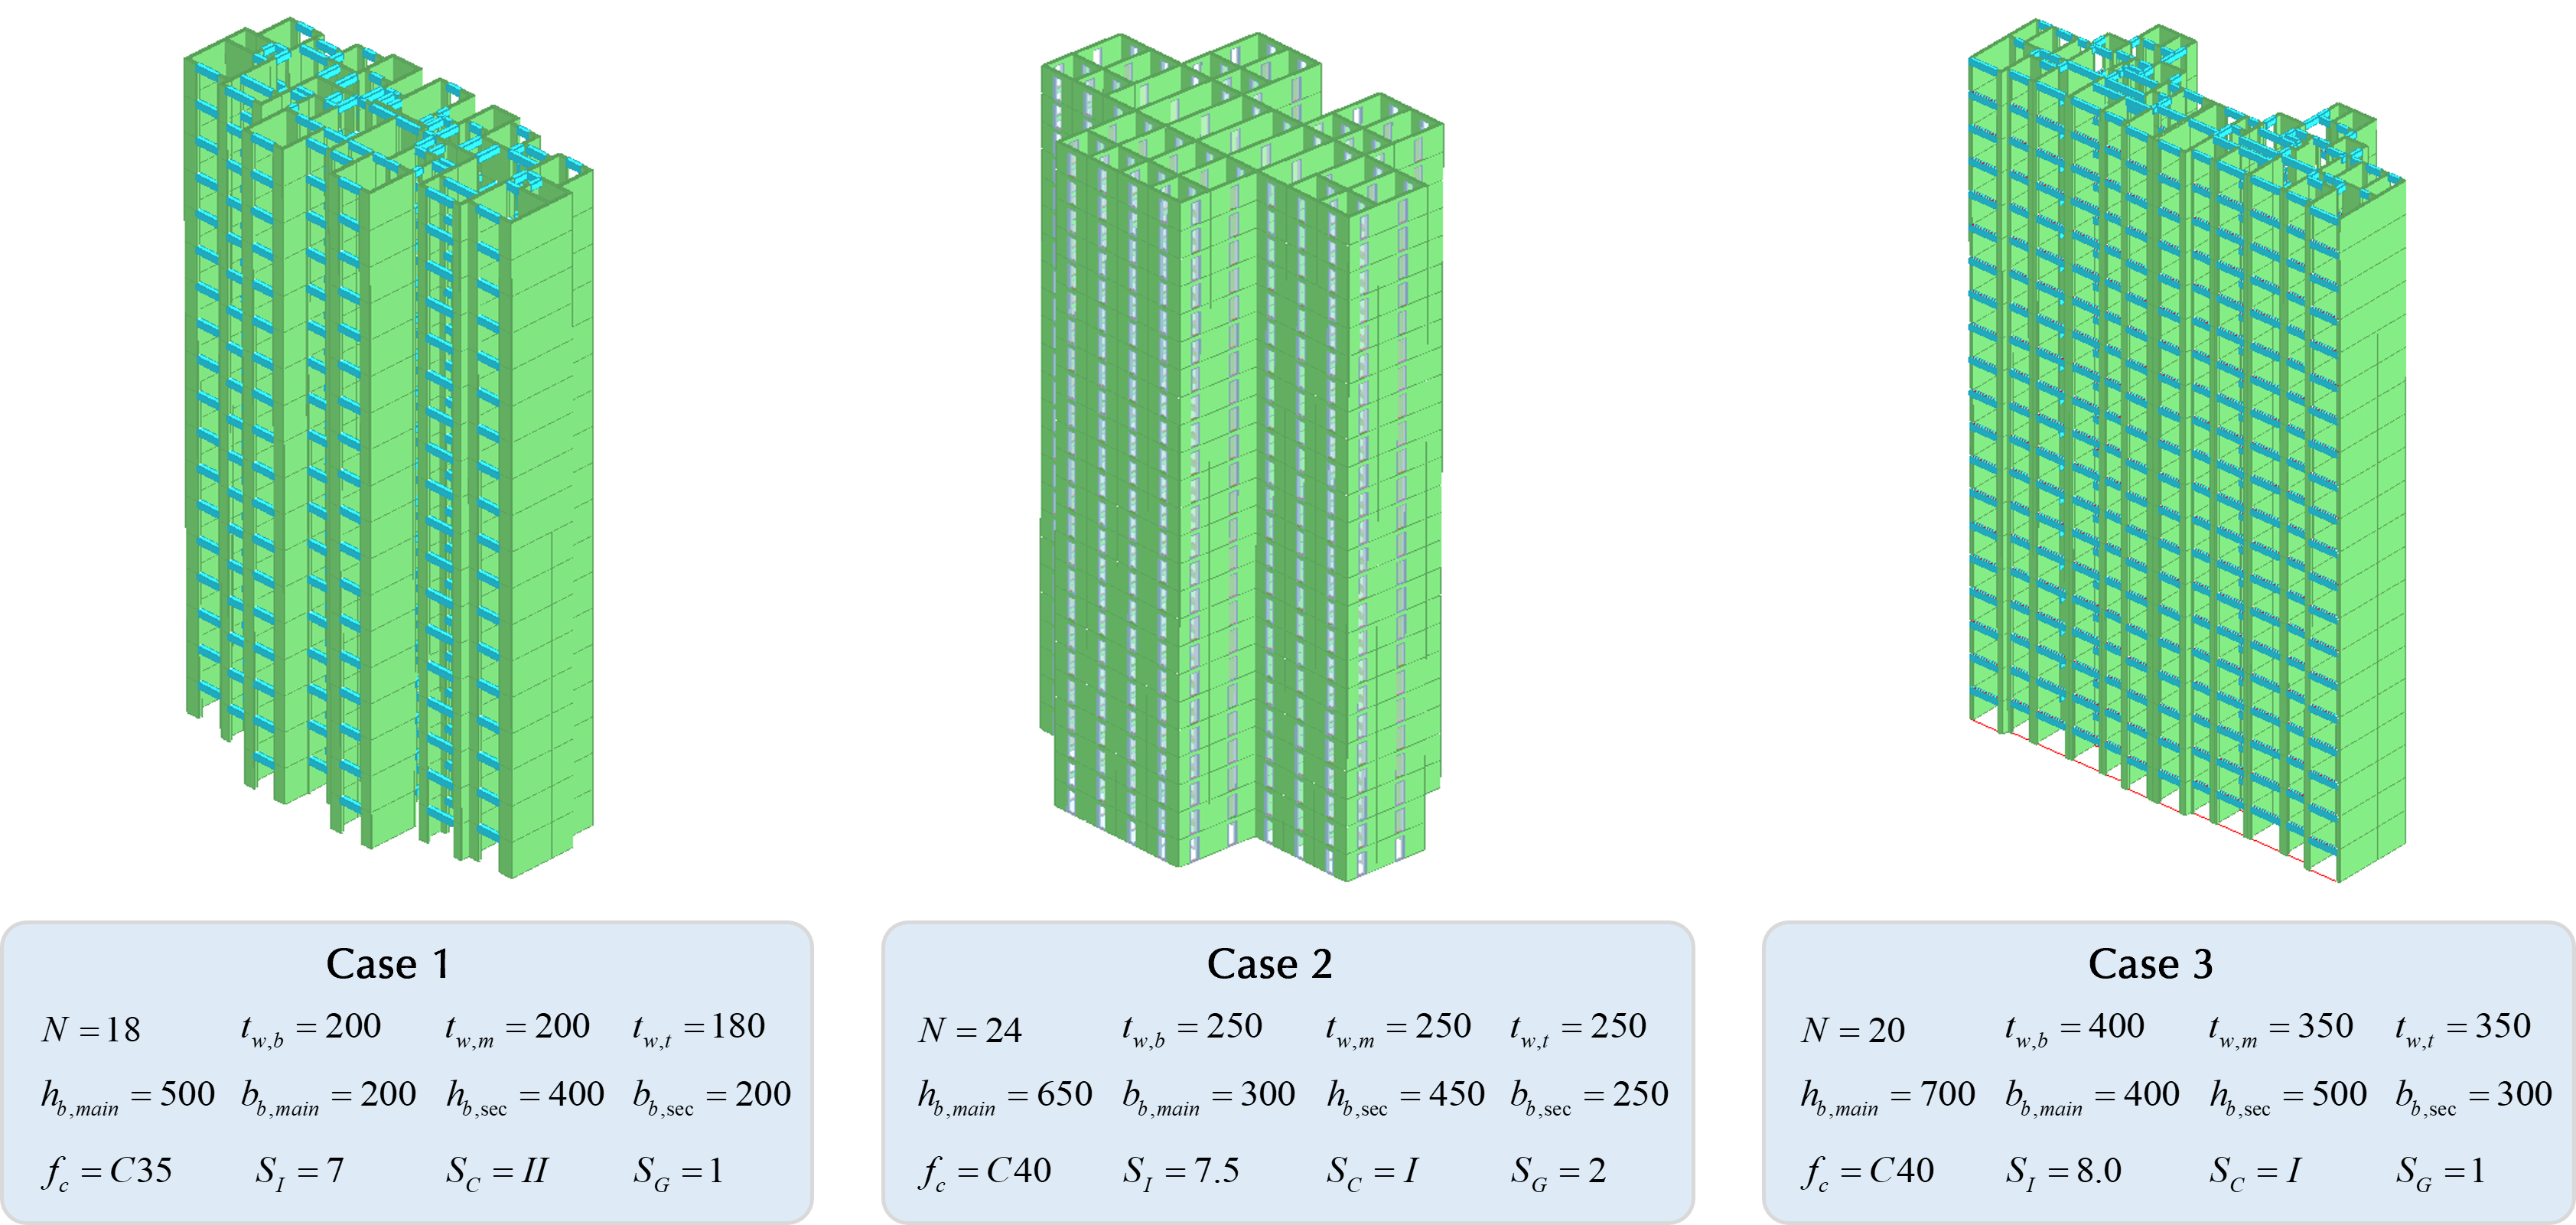
\includegraphics[width=\textwidth]{model_cases.png}
\caption{Representative finite element models of shear wall structures under different sampled design parameters and design conditions.}
\label{fig:model_cases}
\end{figure*}


\begin{figure*}[t]
\centering
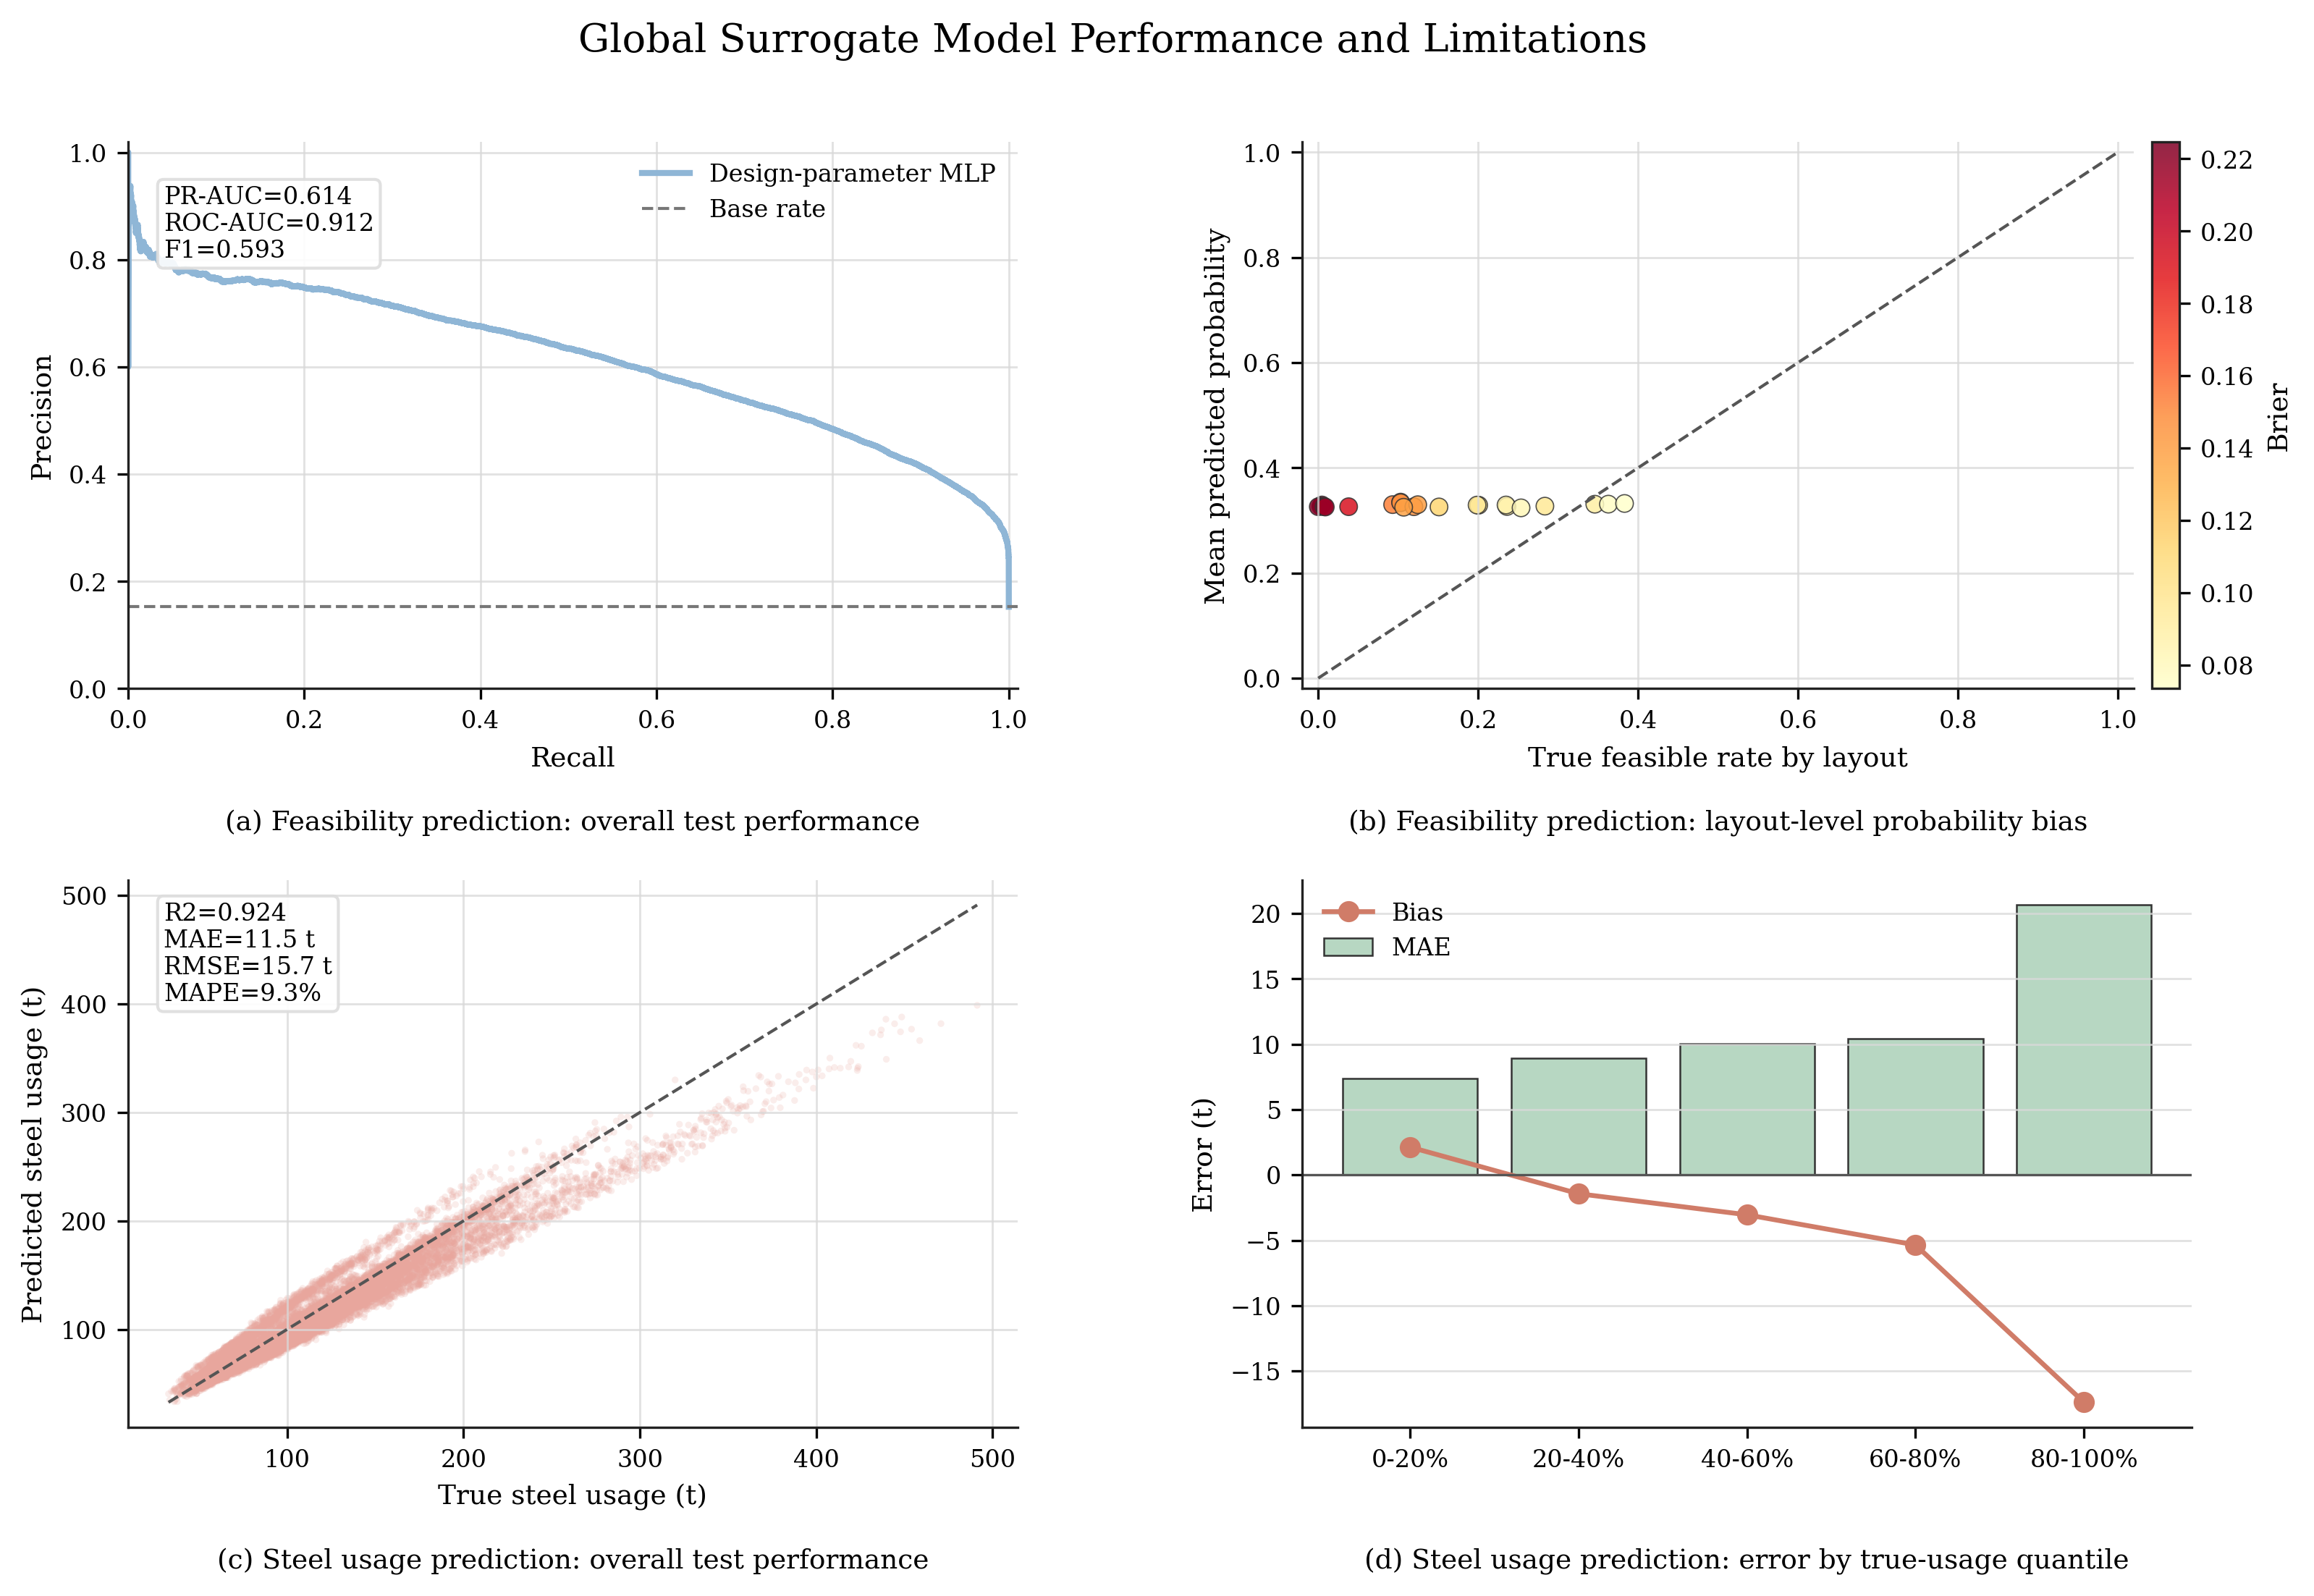
\includegraphics[width=\textwidth]{global_surrogate_overview.png}
\caption{Overall performance and error patterns of the global layout-conditioned surrogate model.}
\label{fig:global_surrogate_overview}
\end{figure*}


\begin{table*}[t]
\centering
\caption{Feasibility prediction performance of different surrogate input settings.}
\label{tab:global_feasibility_results}
\setlength{\tabcolsep}{5pt}
\begin{tabularx}{\textwidth}{@{}>{\raggedright\arraybackslash}X
>{\centering\arraybackslash}p{0.09\textwidth}
>{\centering\arraybackslash}p{0.09\textwidth}
>{\centering\arraybackslash}p{0.07\textwidth}
>{\centering\arraybackslash}p{0.105\textwidth}
>{\centering\arraybackslash}p{0.125\textwidth}
>{\centering\arraybackslash}p{0.145\textwidth}@{}}
\toprule
Model & ROC-AUC & PR-AUC & F1 & Reject rate & Feasible recall & False reject count \\
\midrule
Design-parameter MLP & 0.9117 & 0.6137 & 0.5927 & 0.4787 & 0.9946 & 90 \\
Layout-statistics MLP & 0.9547 & 0.8163 & 0.7370 & 0.4447 & 0.9994 & 10 \\
LayoutParamGNN & 0.9693 & 0.8593 & 0.7688 & 0.4736 & 0.9998 & 3 \\
\bottomrule
\end{tabularx}
\end{table*}


\begin{table*}[t]
\centering
\caption{Reinforcement usage prediction performance of different surrogate input settings.}
\label{tab:global_steel_results}
\setlength{\tabcolsep}{4pt}
\begin{tabularx}{\textwidth}{@{}>{\raggedright\arraybackslash}X
>{\centering\arraybackslash}p{0.075\textwidth}
>{\centering\arraybackslash}p{0.075\textwidth}
>{\centering\arraybackslash}p{0.06\textwidth}
>{\centering\arraybackslash}p{0.07\textwidth}
>{\centering\arraybackslash}p{0.075\textwidth}
>{\centering\arraybackslash}p{0.105\textwidth}
>{\centering\arraybackslash}p{0.09\textwidth}
>{\centering\arraybackslash}p{0.125\textwidth}@{}}
\toprule
Model & MAE (t) & RMSE (t) & $R^2$ & MAPE & Bias (t) & Pairwise acc. & Spearman & Top-10\% recall \\
\midrule
Design-parameter MLP & 32.30 & 45.77 & 0.351 & 0.247 & -13.89 & 0.9586 & 0.9547 & 0.8974 \\
Layout-statistics MLP & 13.83 & 18.75 & 0.891 & 0.112 & -1.66 & 0.9652 & 0.9628 & 0.9142 \\
LayoutParamGNN & 11.48 & 15.67 & 0.924 & 0.093 & -5.02 & 0.9787 & 0.9779 & 0.9483 \\
\bottomrule
\end{tabularx}
\end{table*}


\begin{figure*}[t]
\centering
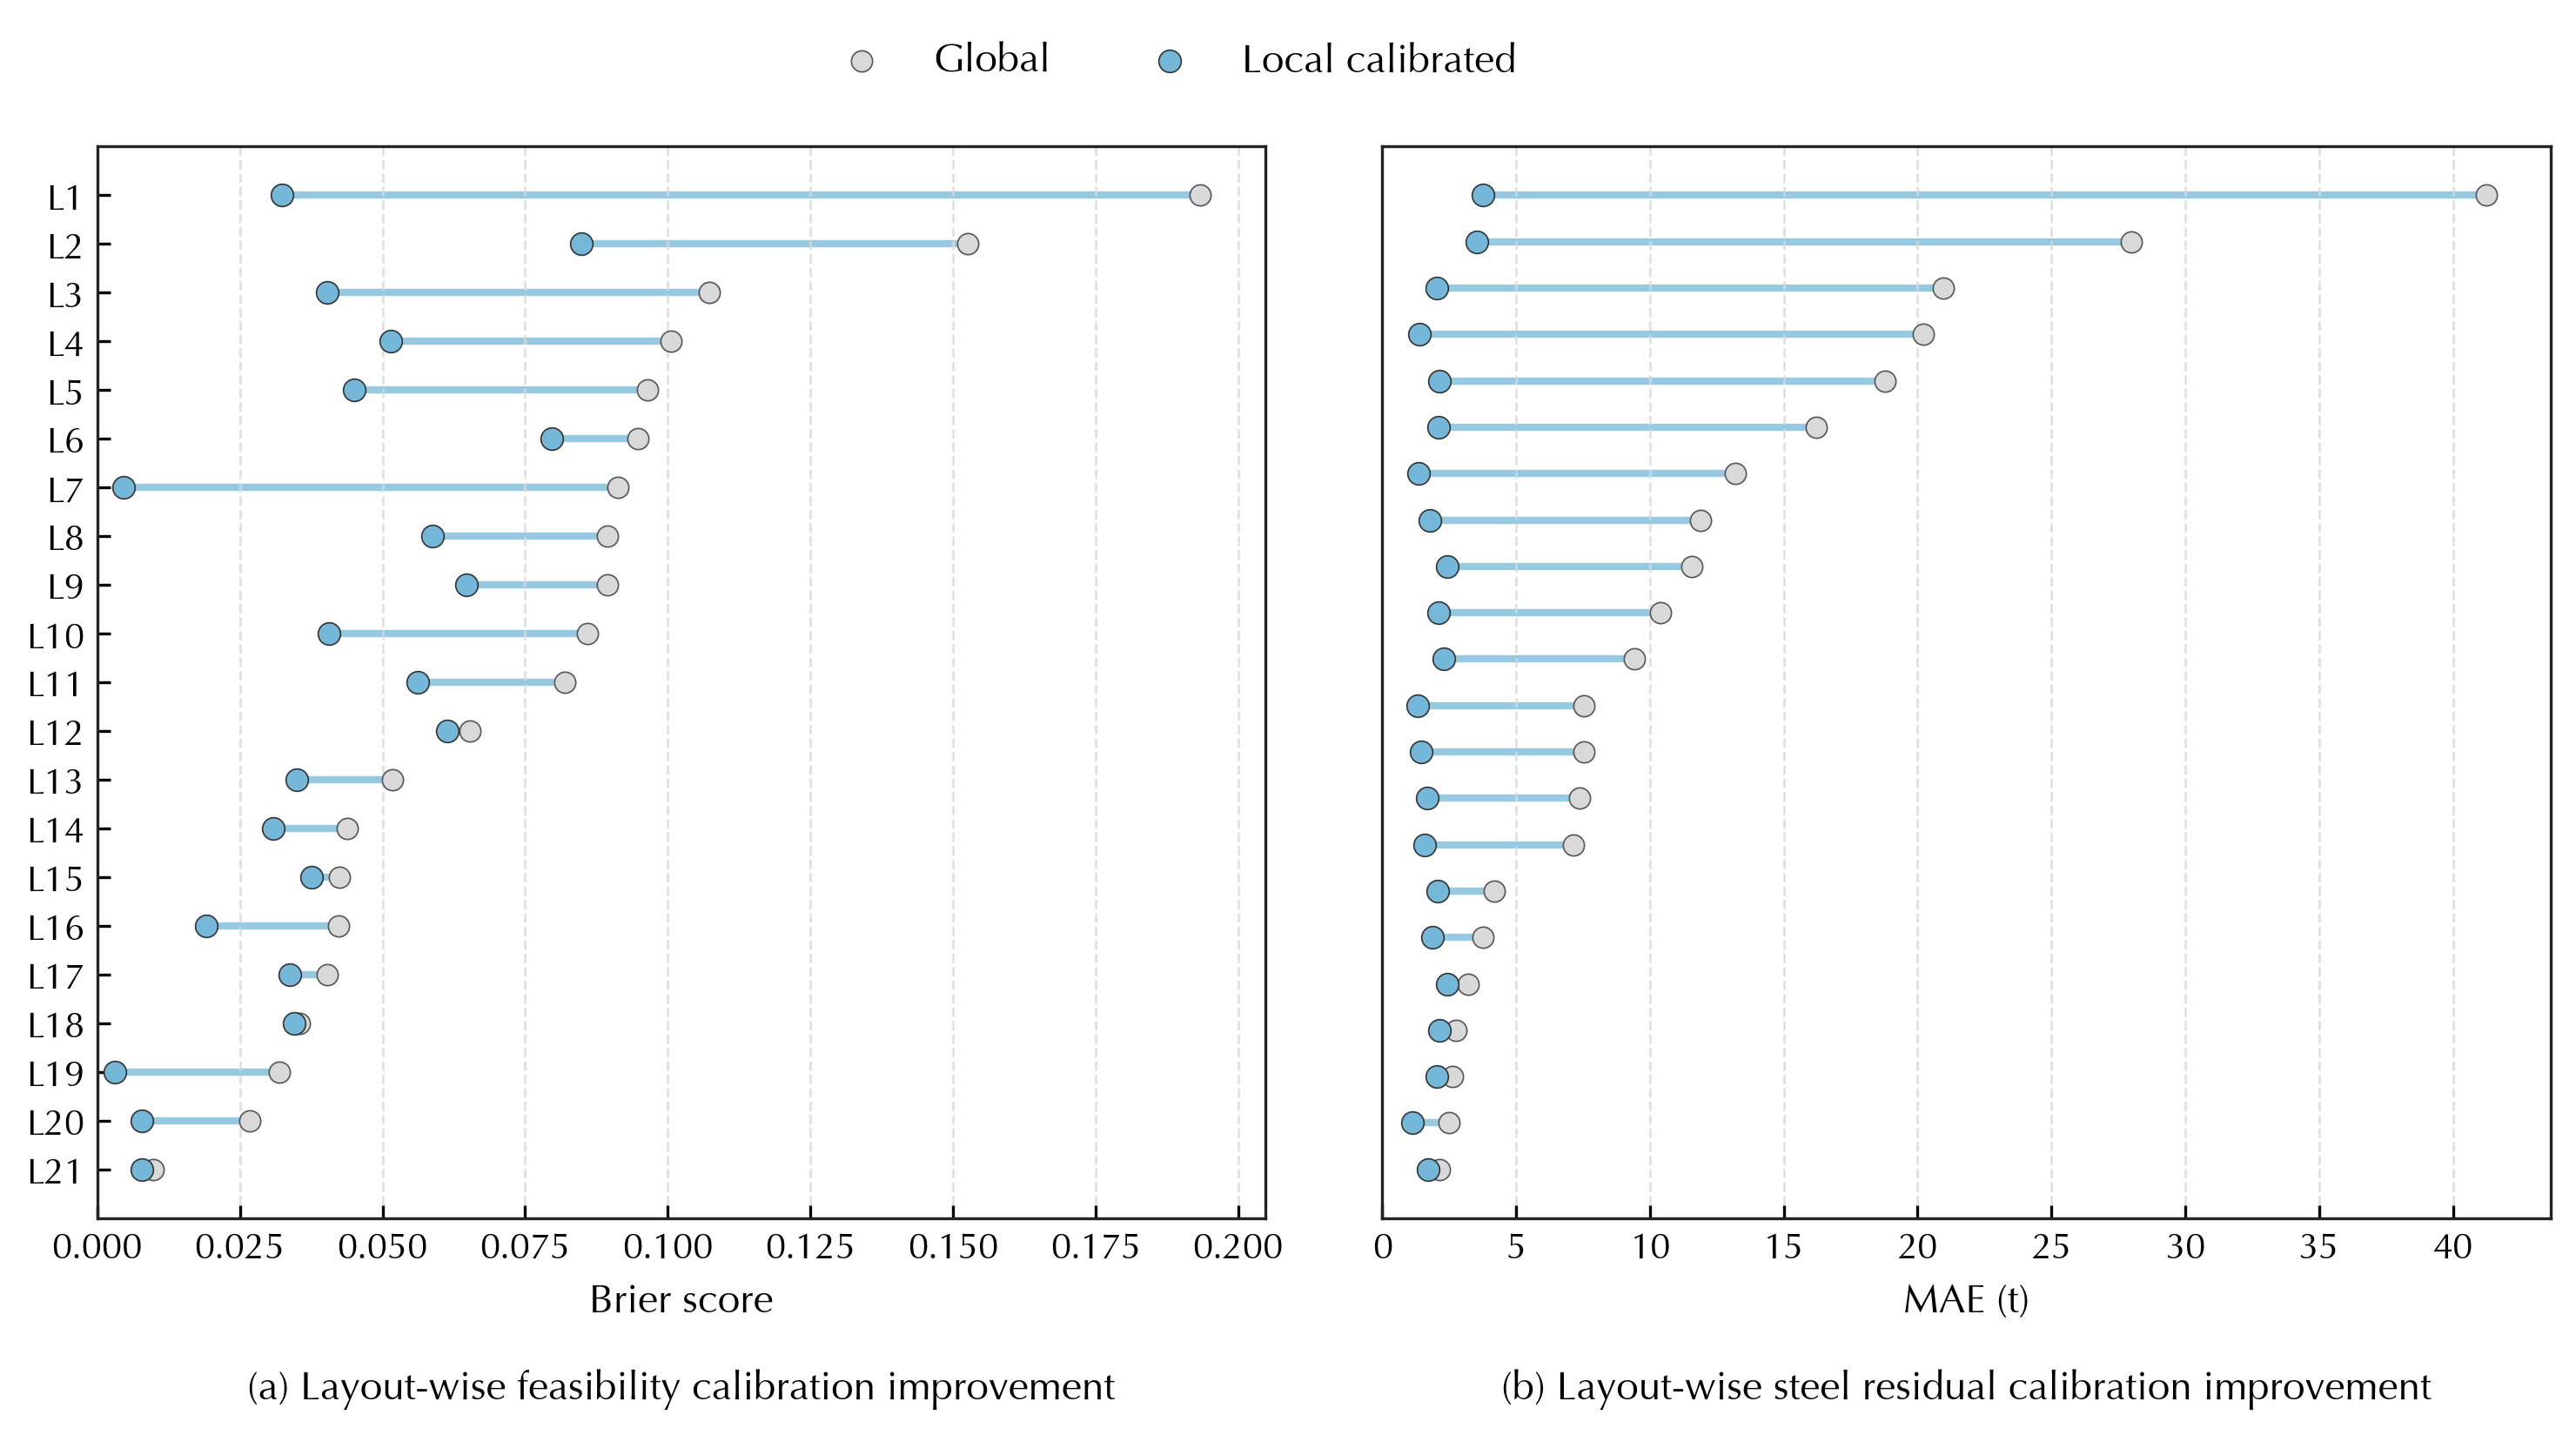
\includegraphics[width=\textwidth]{local_calibration_effect.png}
\caption{Effect of online local calibration using FEA-verified samples from the current layout.}
\label{fig:local_calibration_effect}
\end{figure*}


\begin{table}[t]
\centering
\caption{Representative local calibration results and local-only ablation using 100 FEA-verified samples.}
\label{tab:local_calibration_results}
\setlength{\tabcolsep}{2pt}
\begin{tabularx}{\columnwidth}{@{}>{\raggedright\arraybackslash}X>{\centering\arraybackslash}p{0.14\columnwidth}>{\centering\arraybackslash}p{0.17\columnwidth}>{\centering\arraybackslash}p{0.16\columnwidth}>{\centering\arraybackslash}p{0.13\columnwidth}@{}}
\toprule
Metric & Global & Local only & Calib. & Improv. \\
\midrule
\multicolumn{5}{@{}l}{\textit{Feasibility}} \\
Brier & 0.0749 & 0.0755 & 0.0437 & 42\% \\
ECE & 0.0895 & 0.0451 & 0.0333 & 63\% \\
Screen reject rate & 0.4708 & 0.5639 & 0.5481 & 16\% \\
Screen recall & 0.9990 & 0.7265 & 0.9939 & -1\% \\
\midrule
\multicolumn{5}{@{}l}{\textit{Steel}} \\
MAE & 11.48~t & 4.82~t & 2.04~t & 82\% \\
RMSE & 12.30~t & 5.64~t & 2.76~t & 78\% \\
$R^2$ & 0.847 & 0.976 & 0.994 & 17\% \\
MAPE & 9.26\% & 3.26\% & 1.64\% & 82\% \\
\bottomrule
\end{tabularx}
\end{table}


\begin{figure*}[t]
\centering
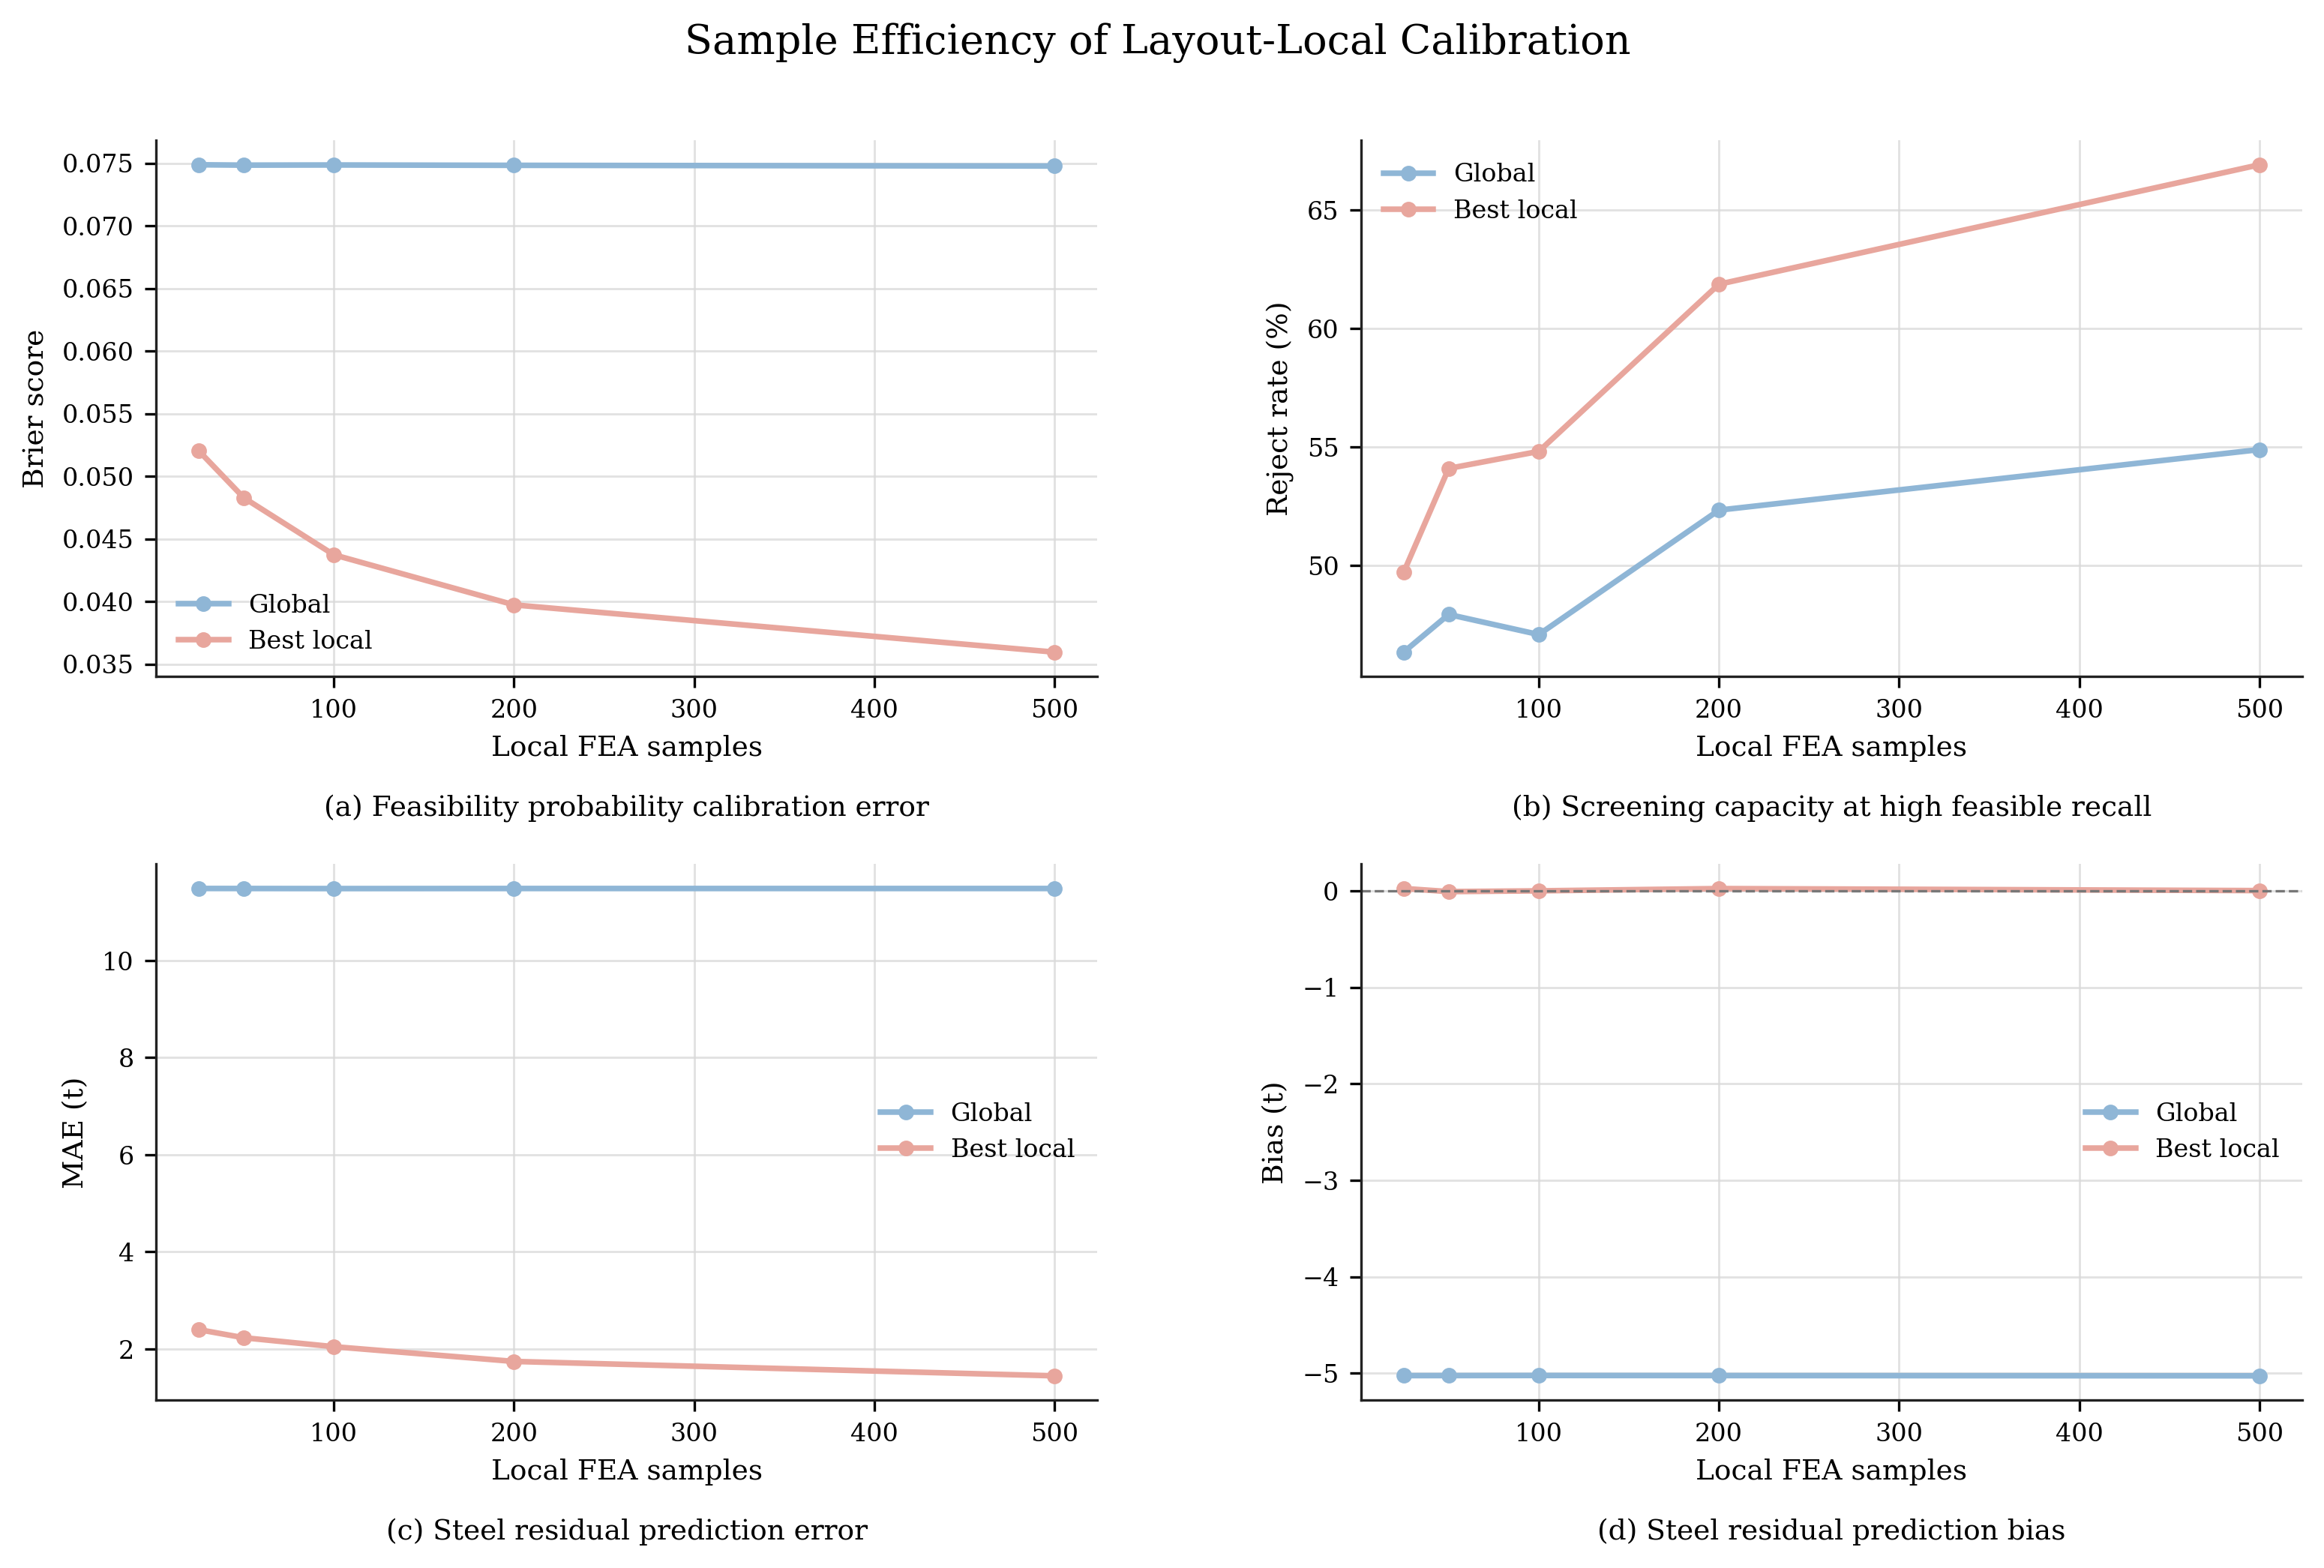
\includegraphics[width=\textwidth]{calibration_sample_efficiency.png}
\caption{Sample efficiency of online local calibration under different numbers of local FEA-verified samples.}
\label{fig:calibration_sample_efficiency}
\end{figure*}

\subsection{Dataset and Structural Evaluation}
\label{subsec:dataset_structural_evaluation}

The dataset is constructed from engineering shear wall layouts and a parametric structural evaluation workflow. Each sample corresponds to a layout, a design condition, and a section-material design scheme. The input includes layout information and design parameters, and the supervised labels include the comprehensive feasibility label $y_f$ and the reinforcement usage $m_s$.

The dataset contains 143 shear wall layouts designed by professional engineers, which can be divided into three groups according to seismic intensity and building height. Group7-H1 corresponds to low-demand cases with seismic intensity 7, PGA of 0.10~g, and building height $H \leq 50$~m. Group7-H2 corresponds to medium-demand cases with the same seismic intensity but building height $H>50$~m. Group8 corresponds to high-demand cases with seismic intensity 8 and PGA of 0.20~g. These groups reflect the combined influence of seismic demand and structural height on shear wall section design and material usage.

For each layout, 5000 candidate design schemes are sampled from a predefined parameter space, which is summarized in Table~\ref{tab:parameter_space}. The sampled variables include the number of stories, wall thicknesses in different vertical zones, main and secondary beam dimensions, concrete strength grade, seismic intensity, site class, and seismic group. During sampling, wall thicknesses are constrained to be nonincreasing along the building height, i.e., $t_{w,t}\le t_{w,m}\le t_{w,b}$.

Representative finite element models generated from the same parametric workflow are shown in Fig.~\ref{fig:model_cases}.


A true structural evaluator $\mathcal{E}$ is used to generate labels for all sampled candidates. For each candidate, the evaluator automatically constructs the structural model, performs FEA in OpenSees\cite{McKenna2011OpenSees}, extracts global structural responses and member forces, and conducts code-based member design and reinforcement calculation. The comprehensive feasibility label $y_f$ is determined by analysis validity, global response limits, and member-level design checks. The reinforcement usage label $m_s$ is obtained from the final member design results.

The resulting dataset contains 715,000 FEA-labeled samples. After removing cases with failed analyses or invalid results, the final dataset contains 714,972 samples. A layout-level split is adopted to evaluate cross-layout generalization. Specifically, 100 layouts are used for training, 21 layouts for validation, and 22 layouts for testing, corresponding to an approximate ratio of 0.70:0.15:0.15. All parameter variants of the same layout are assigned to the same subset to avoid information leakage between training and testing. The test layouts cover the three design-condition groups and are used for global surrogate evaluation, local calibration analysis, and optimization benchmarking.

 The detailed distribution of layouts and samples across design-condition groups is given in Table~\ref{tab:dataset_split}.


\subsection{Global Surrogate Model Training}
\label{subsec:global_surrogate_training}

Two global surrogate models are trained, i.e. the feasibility surrogate $SM_f$ and the reinforcement usage surrogate $SM_s$. They use the same candidate representation and model architecture, but are trained separately with independent parameters for different prediction tasks. The feasibility surrogate outputs the probability that a candidate can pass the comprehensive structural checks, while the reinforcement surrogate predicts the reinforcement quantity before true evaluation.

To examine the effect of layout representation, three model settings are compared. The Design-parameter MLP uses only section, material, and design-condition parameters, the Layout-statistics MLP further incorporates global layout statistics, and the LayoutParamGNN jointly uses the room-level graph, global layout statistics, and design parameters. Here, global layout statistics refer to fixed-dimensional tabular descriptors computed from the overall shear wall layout, such as plan aspect ratio, shear wall ratio, total wall length, centroid-related measures, and other geometric summaries, which convert layouts with variable numbers of wall components into fixed-length features.

The LayoutParamGNN adopts a three-layer GraphSAGE encoder for room-graph feature extraction\cite{Hamilton2017GraphSAGE}. In each surrogate model, the graph-level representation is fused with global layout statistics and design-parameter embeddings before being passed to the task-specific output layer. For the feasibility model, the hidden dimension, dropout rate, batch size, and learning rate are set to 256, 0.2, 128, and 0.001, respectively. Weighted binary cross-entropy is used to handle class imbalance. The screening threshold is selected on the validation set according to a target feasible recall of 0.995, and the default classification threshold of 0.5 is not used.

For the reinforcement model, the hidden dimension, dropout rate, batch size, and learning rate are set to 128, 0.1, 512, and 0.0005, respectively. Both global surrogate models are trained using validation-based early stopping.


\subsection{Local Calibration Settings}
\label{subsec:local_calibration_settings}

Local calibration experiments are conducted on the test layouts to simulate the use of FEA-verified samples accumulated during optimization. For each test layout, a certain number of verified samples are randomly selected as the local calibration set, and the remaining samples are used as the layout-specific evaluation set. Each local calibration sample stores the candidate representation, the global surrogate predictions, and the true FEA-based labels.

The calibration objects are the feasibility probability and the reinforcement residual. For feasibility calibration, the global feasibility probability is first transformed into the logit space and then combined with the design parameters as the calibration input, while the target is the true feasibility label. Several lightweight calibration methods are compared, including Platt scaling\cite{Platt1999} and isotonic regression\cite{Zadrozny2002}. In addition, residual-based probability correction and ensemble voting/averaging are tested as simple empirical alternatives for local probability adjustment \cite{Bella2013}. The calibrated probabilities are used to assess probability reliability and conservative screening performance.

For reinforcement calibration, the model learns the residual between the true reinforcement usage and the global surrogate prediction. The input consists of the global reinforcement prediction and design parameters, while the target is the reinforcement residual. Ridge regression\cite{Hoerl1970Ridge}, Gaussian process regression\cite{Rasmussen2006GPML}, LightGBM\cite{Ke2017LightGBM}, and K-nearest neighbors\cite{Cover1967KNN} are compared as lightweight residual calibration models. These comparisons test whether the systematic error of the global model can be corrected with a small number of layout-specific FEA samples.

To examine sample efficiency, local calibration sizes of 25, 50, 100, 200, and 500 samples are considered. Each setting is repeated three times with different random samples, and the average results are reported. In the online optimization experiments, local calibration is activated only after at least 25 FEA-verified samples have been accumulated for the current layout. The feasibility screening threshold follows the same conservative principle as the global model, with a target feasible recall of 0.995 and a threshold scale factor of 0.1. When the local samples are insufficient or contain only one class for the feasibility task, the framework falls back to the global surrogate prediction and the validation-based global threshold.

\subsection{Optimization Benchmark Settings}
\label{subsec:optimization_benchmark_settings}

Optimization experiments are conducted on 15 unseen layouts selected from the test set, with five layouts from each design-condition group. For each layout, five random seeds are used. For each test layout, the layout $L$ and design condition $c$ are fixed, and the optimization variables are the section and material parameters $x$. All compared methods use the same design space, true evaluator, and random seeds.

Genetic algorithm is adopted as the main optimizer\cite{Goldberg1989}. In the experiments, the population size, number of generations, mutation rate, and elite size are set to 48, 15, 0.30, and 2, respectively. To examine whether the surrogate-assisted mechanism depends on a specific optimizer, particle swarm optimization (PSO) and random search are also included as supplementary optimizers\cite{Kennedy1995PSO}. The PSO uses a swarm size of 48 and 15 iterations, with a mutation rate of 0.15 to improve exploration. The random search baseline evaluates 720 candidates in batches of 48.

Three candidate evaluation strategies are compared:
\begin{enumerate}
\item \textbf{Full FEA optimization}: all candidates generated by the optimizer are evaluated by $\mathcal{E}$. This strategy serves as the baseline.
\item \textbf{Cost ranking}: candidates are ranked using the reinforcement surrogate and the estimated concrete quantity, and only high-priority candidates are submitted to $\mathcal{E}$.
\item \textbf{Screen \& cost ranking}: feasibility screening, reinforcement-based cost ranking, and online local calibration are jointly used to select candidates for true FEA evaluation.
\end{enumerate}

For surrogate-assisted strategies, each optimizer first generates a candidate batch $\mathcal{B}_t$. The surrogate module then evaluates all candidates in the batch and selects a subset $\mathcal{S}_t$ for true FEA and code checking. A minimum number of evaluated candidates is enforced to avoid overly aggressive filtering. In the experiments, the minimum number of true evaluations per batch is set to \texttt{min\_eval} = 8. The verified results are used to update the optimizer and the local calibration set. Candidates not selected for FEA are not used as true samples and are not considered in final best-solution comparison.

The cost-ranking uses an evaluation ratio of 0.8 before the first feasible design is found and 0.5 afterwards. After a feasible design has been observed, the selected subset is allocated to cost ranking, feasibility-risk ranking, and random exploration with ratios of 0.60, 0.25, and 0.15, respectively. The feasibility-risk term in the surrogate ranking score uses a hinge target of $p_0=0.5$ and a penalty coefficient of $\eta=1.0\times10^6$. Candidates rejected by surrogate screening or skipped after cost ranking are assigned $M_{rej}=1.0\times10^{12}$. For FEA-evaluated infeasible candidates, the scalar penalty uses $P_0=1.0\times10^5$, $\lambda_v=1.0\times10^7$, and $\lambda_c=0.01$.

\subsection{Evaluation Metrics}
\label{subsec:evaluation_metrics}

Definitions of the full set of metrics used in this study are provided in \ref{app:evaluation_metrics}.

The feasibility surrogate is assessed using ROC-AUC, PR-AUC, and F1 score to characterize overall classification performance. Because it is used as a conservative screening tool, feasible recall, reject rate, and false reject count are also reported to quantify the retained feasible candidates, the candidates filtered before FEA, and the feasible candidates mistakenly rejected by the screen.

Reinforcement prediction accuracy is measured by mean absolute error (MAE), root mean square error (RMSE), coefficient of determination ($R^2$), mean absolute percentage error (MAPE), and bias. To reflect its role in candidate ranking, pairwise ranking accuracy, Spearman correlation, and top-$k$ recall are further included.

Local calibration is evaluated from both probability and residual-correction perspectives. Feasibility probability calibration is measured by Brier score\cite{Brier1950} and expected calibration error (ECE)\cite{Naeini2015}, together with screening recall and reject rate, whereas reinforcement residual calibration is measured by MAE, RMSE, bias, and the ranking metrics after calibration.

Optimization performance is summarized in terms of computational efficiency and solution quality. Efficiency is measured by the number of true FEA calls and the FEA reduction ratio, while solution quality is characterized by feasible-solution discovery rate, the number of FEA calls required to find the first feasible solution, and final material cost. For each test layout and random seed, surrogate-assisted strategies are compared with full FEA optimization to determine whether FEA calls can be reduced without substantial degradation in feasibility discovery or final cost.
